%%
%% This is file `example.tex',
%% generated with the docstrip utility.
%%
%% The original source files were:
%%
%% aobs-tikz.dtx  (with options: `example')
%% * * * * * * * * * * * * * * * * * * * * * * * * * * * * * * * * * * * * * * * *
%% aobs-tikz - TikZ auxiliary styles for Beamer overlays
%% 
%% E-mail: claudio dot fiandrino at gmail dot com
%% 
%% Released under the LaTeX Project Public License v1.3c or later
%% See http://www.latex-project.org/lppl.txt
%% * * * * * * * * * * * * * * * * * * * * * * * * * * * * * * * * * * * * * * * *
%% 
%% The package defines auxiliary TikZ styles useful for
%% overlaying pictures' elements in Beamer.
%% 
%% The TikZ styles are grouped in a library, overlay-beamer-styles
%% which is automatically called by the aobs-tikz package. Users
%% can either load only aobs-tikz or the library; the latter method
%% necessitates TikZ manual load.
\documentclass{beamer}
\usepackage{lmodern}
\usepackage{tikz}
\usetikzlibrary{positioning,
  shapes.geometric,
  shadows
}
\usetikzlibrary{overlay-beamer-styles}

\definecolor{processblue}{cmyk}{0.96,0,0,0}

\begin{document}
\begin{frame}{Styles for draw, fill and shading modifications}
\begin{columns}[T]
\begin{column}{0.2\textwidth}
\centering
Fill draw\\[2ex]
\tikz[baseline=(A.base)]{%
\node[background fill=red!50,%
      fill on=<2>,%
      anchor=base,%
      rounded corners,%
      ] (A) {ABCD};
}

\tikz[baseline=(A.base)]{%
\node[background fill=blue!50,%
      fill on=<{1,3}>,%
      anchor=base,%
      rounded corners,%
      ] (A) {EFGH};
}

\tikz[baseline=(A.base)]{%
\node[background draw=red,%
      draw on=<2>,%
      anchor=base,%
      rounded corners,%
      ] (A) {IJKL};
}

\tikz[baseline=(A.base)]{%
\node[background draw=blue,%
      draw on=<{1,3}>,%
      anchor=base,%
      rounded corners,%
      ] (A) {MNOP};
}

\tikz[baseline=(A.base)]{%
\node[background filldraw=red filled by blue!10,%
      filldraw on=<2>,anchor=base,%
      rounded corners,%
      ] (A) {QRST};
}
\end{column}
\begin{column}{0.2\textwidth}
\centering
Shadings\\[2ex]
\tikz[baseline=(A.base)]{%
\node[background shade={top color=red!50, bottom color=white},%
      shade on=<2>,%
      anchor=base,%
      rounded corners,%
      ] (A) {ABCD};
}

\tikz[baseline=(A.base)]{%
\node[background shade={inner color=red!50, outer color=white},%
      shade on=<{1,3}>,%
      anchor=base,%
      rounded corners,%
      ] (A) {EFGH};
}

\tikz[baseline=(A.base)]{
\node[background shade={left color=orange!50, right color=white},%
      shade on=<2>,%
      anchor=base,%
      rounded corners,%
      ] (A) {IJKL};
}

\tikz[baseline=(A.base)]{
\node[background shadedraw={blue}{top color=white, bottom color=cyan!30},%
      shadedraw on=<{1,3}>,%
      anchor=base,%
      rounded corners,%
      ] (A) {MNOP};
}

\tikz[baseline=(A.base)]{
\node[background shadedraw={green!50!black}{inner color=white,%
      outer color=green!30},%
      shadedraw on=<2>,%
      anchor=base,%
      rounded corners,%
      ] (A) {QRST};
}
\end{column}
\begin{column}{0.55\textwidth}
\centering
Node application\\[2ex]
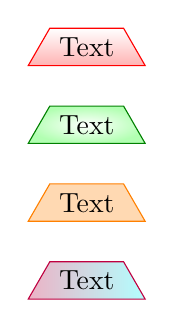
\begin{tikzpicture}[node distance=0.5cm]
\tikzset{visibility 1/.style={
      background draw=red, draw on=<{1,4}>,
      background shade={top color=white,
      bottom color=red!30},
      shade on=<{2,3}>,
      }
}
\tikzset{visibility 2/.style={
      background shadedraw={green!50!black}{inner color=white,
      outer color=green!30},
      shadedraw on=<{2,3}>,
      }
}
\tikzset{visibility 3/.style={
      background draw=orange,
      draw on=<1->,
      background fill={orange!30},
      fill on=<{2,3}>,
    }
}
\tikzset{visibility 4/.style={
      background draw=purple,
      draw on=<2->,
      background shade={left color=purple!30,
      right color=cyan!30},
      shade on=<{3,4}>,
    }
}
\node[trapezium,
      visibility 1] (A) {Text};
\node[trapezium,
      visibility 2,
      below= of A] (B) {Text};
\node[trapezium,
      visibility 3,
      below= of B] (C) {Text};
\node[trapezium,
      visibility 4,
      below= of C] (D) {Text};
\end{tikzpicture}
\end{column}
\end{columns}
\end{frame}

\begin{frame}{Styles for path aspect and text color modifications}
\centering
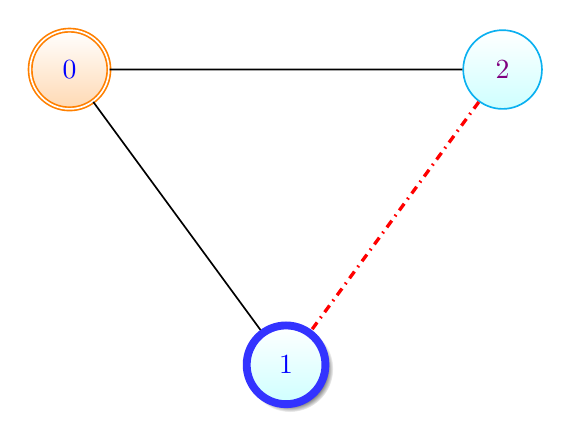
\begin{tikzpicture}[node distance=3cm and 2cm,
      semithick ,
      state/.style={circle,
            top color=white,
            bottom color=processblue!20,
            draw, processblue,
            text=blue,
            minimum width=1cm},
      background default shade={top color=white,
            bottom color=processblue!20},
      background default draw={processblue,
            semithick}]
\node[state,
      background draw={blue!80,
            line width=1mm},
      draw on=<2>,
      circular drop shadow={visible on=<2>},
      visible on=<{1,2}>% NOT visible in 3
     ] (C) {$1$};
\node[state,
      background draw={orange},
      draw on=<{1,3}>,
      background default aspect={semithick,
            double disabled},
      background aspect={double},
      aspect on=<{1,3}>,
      background shade={top color=white,
            bottom color=orange!30},
      shade on=<{1,3}>,
      above left= of  C] (A) {$0$};

\node[state,
      background text=violet,
      background default text=red,
      text on=<2>,
      above right= of C] (B) {$2$};

\draw (A)-- (B) (C)-- (A);

\draw[background default aspect={solid,semithick},
      background aspect={dashdotted,
            very thick},
      aspect on=<{2,3}>,
      background default draw={black},
      background draw={red},
      draw on=<3>](B)-- (C);
\end{tikzpicture}
\end{frame}
\end{document}
%% 
%% Copyright (C) 2014 by Claudio Fiandrino <claudio.fiandrino@gmail.com>
%% 
%% This file may be distributed and/or modified under the conditions
%% of the LaTeX Project Public License, either version 1.3 of this
%% license or (at your option) any later version.
%% The latest version of this license is in:
%% 
%%    http://www.latex-project.org/lppl.txt
%% 
%% and version 1.3 or later is part of all distributions of LaTeX
%% version 2005/12/01 or later.
%% 
%% This work is "maintained" (as per LPPL maintenance status) by
%% Claudio Fiandrino.
%% 
%% This work consists of the files  aobs-tikz.dtx
%% and the derived files  aobs-tikz.ins
%%                                  aobs-tikz.sty
%%                                  tikzlibrarybeamer-overlay-styles.code.tex
%%                                  aobs-tikz.pdf
%%                                  example.tex
%%                                  example.pdf
%%                                  README.txt
%% 
%%
%% End of file `example.tex'.
